\documentclass{beamer}
\usefonttheme[onlymath]{serif}
\usetheme{Boadilla}
\usepackage{amsmath}
\usepackage{mathtools}
\title{Introduction to Neural Networks}
\subtitle{Day 3}
\author{Mohammad Khajah}
\institute[KISR]{Kuwait Institute for Scientific Research}
\date{}

\begin{document}

\begin{frame}
\titlepage
\end{frame}

\begin{frame}
\frametitle{Topics to Cover}

\begin{itemize}
\item Automatic differentiation with Tensorflow
\item Neural Networks
\item Overfitting and generalization
\item Regularization
\end{itemize}

\end{frame}

\begin{frame}
\frametitle{An Artificial Neuron}
 \begin{figure}
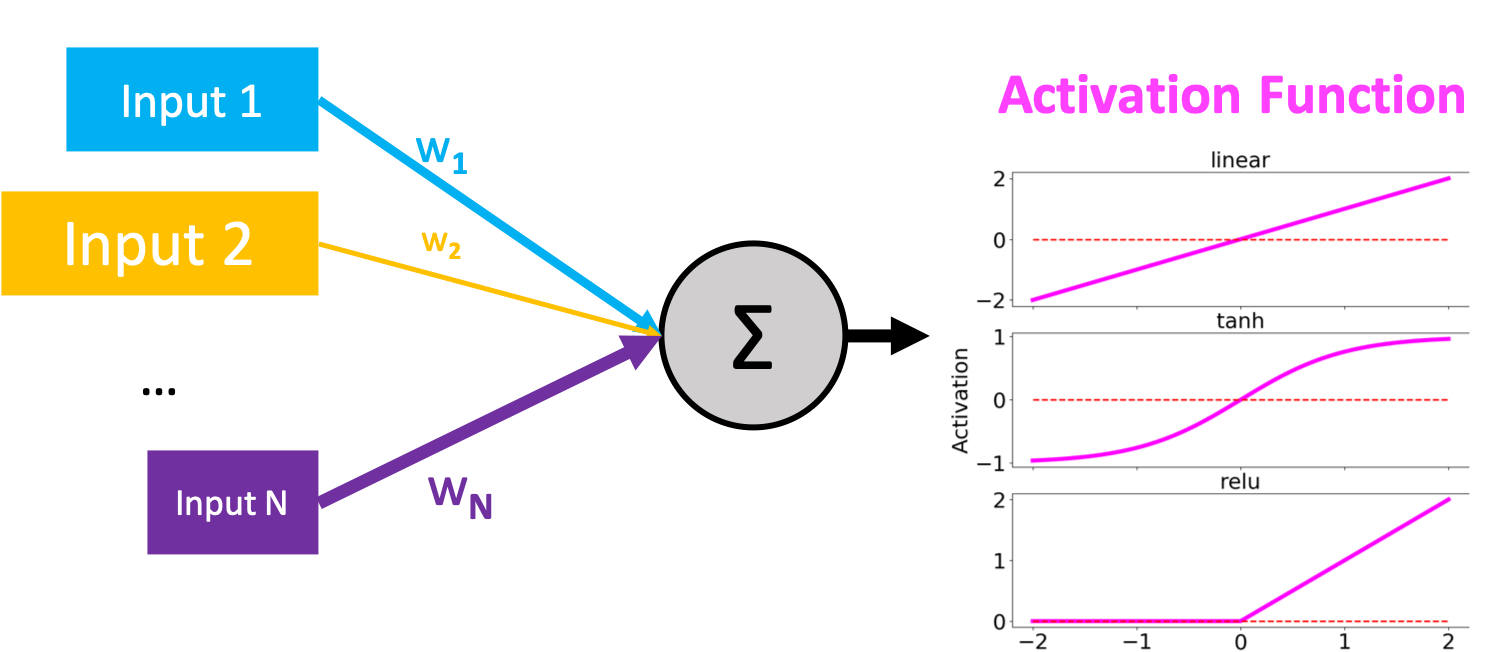
\includegraphics[width=\textwidth]{../figures/neuron.png}
\end{figure}
\end{frame}

\end{document}